\documentclass[fleqn]{article}
\usepackage[utf8]{inputenc}
\usepackage{amsmath}
\usepackage{amsfonts}
\usepackage{amssymb}
\usepackage{graphicx}
\usepackage{fancyhdr}
\usepackage{tabularx}
\usepackage{geometry}
\usepackage{setspace}
\usepackage[right]{eurosym}
\usepackage[printonlyused]{acronym}
\usepackage{subfig}
\usepackage{floatflt}
\usepackage[usenames,dvipsnames]{color}
\usepackage{colortbl}
\usepackage{paralist}
\usepackage{array}
\usepackage{titlesec}
\usepackage{parskip}
\usepackage[right]{eurosym}
%\usepackage{picins}
\usepackage[subfigure,titles]{tocloft}
\usepackage[pdfpagelabels=true]{hyperref}
\usepackage{mathdots}
\usepackage{listings}
\usepackage{lipsum}
\usepackage{booktabs}
\usepackage{fix-cm}
\usepackage[labelfont=bf]{caption}
\captionsetup{labelfont=bf}
%opening
\title{\textbf{15D013} Topics in Big Data Analytics II - Problem Set 1 - Computational Finance}
\author{Felix Gutmann}

\begin{document}

\maketitle

%---------------------------------------------------------------------------------------------------------------
% Prerequisites 
%---------------------------------------------------------------------------------------------------------------

\section*{Prerequisites}
In the following we will apply the following notation. Let $R_t$ be the returns of a stock series defined as follows:
\begin{flalign}
R_t&:= \frac{P_t}{P_{t-1}} - 1, \nonumber
\intertext{where $P_t$ is the price of the stock at time $t$. In comparrison to that let $r_t$ be the log returns of a series $P$ defined as:}
r_t&:= \log R_t =  \log \left( \frac{P_t}{P_{t-1}} - 1 \right) = \log( P_t ) -\log( P_{t-1} ) \nonumber
\end{flalign}
\pagebreak
%---------------------------------------------------------------------------------------------------------------
% Exercise 1 
%---------------------------------------------------------------------------------------------------------------


\section*{Exercise 1}

Figure (1) depicts the the different acf values for the powers of the absolute returns series of the adjusted closing price of GOOGLE displaying the \textit{Taylor-Effect}. 

\begin{figure}[!htb]
	\centering
	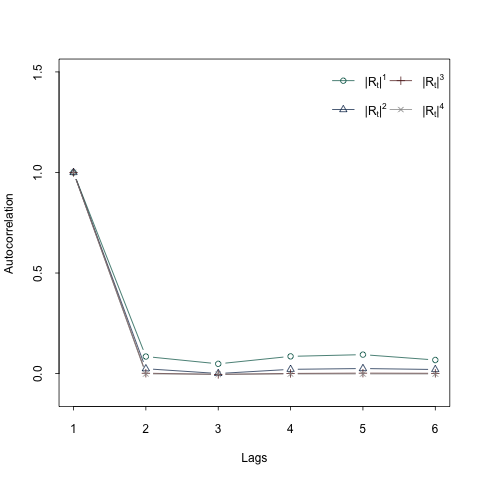
\includegraphics[width=\textwidth]{p1.png}
	\caption{Autorrelations for $|R_t|^{k}$ for adjusted GOOGLE closing price (k=(1,$\dots$,4))}
\end{figure}
 
\pagebreak

%---------------------------------------------------------------------------------------------------------------
% Exercise 2
%---------------------------------------------------------------------------------------------------------------

\section*{Exercise 2}

Figure (2) depicts the monthly \textit{Michigan Consumer Sentiment Index} (MCSI) from 01.01.1978 - 01.04.2016. 

\begin{figure}[!htb]
\centering
	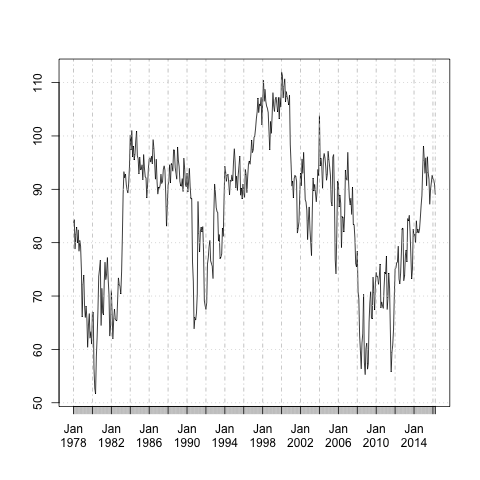
\includegraphics[width=\textwidth]{p2.png}
\caption{Michigan Consumer Sentiment Index (01.01.1978 - 01.04.2016) }
\end{figure}
\pagebreak
Figure (3) displays the ACF (sub-figure (a)) and the PACF (sub-figure(b)) of the returns of the MCSI. We can observe that we may have a weak autoregressive component of order one (at most) and a moving average component.  Conducting an \textit{Augmented-Dicky-Fuller} test (ADF-test) ensures that the returns are stationary (see listing (3) in the appendix). The ARMA fitted by auto.arima() is an ARMA(1,2) (see listing (4) in the appendix) .

\begin{figure}[!htb]
\centering
\begin{tabular}{cc}
		
\includegraphics[width=60mm]{p3.png} &   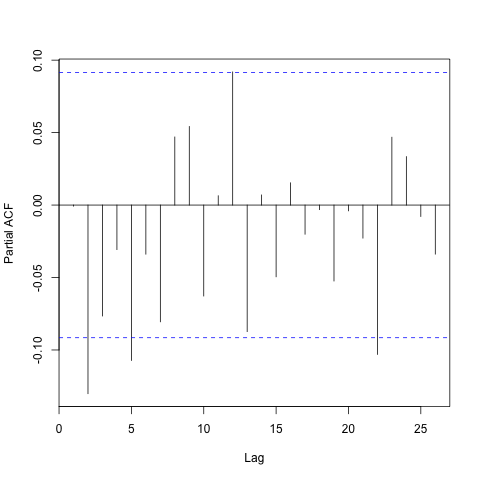
\includegraphics[width=60mm]{p4.png} \\
		(a) ACF  & (b) PACF  \\[4pt]
\end{tabular}
\caption{ACF and PACF of MCSI}
\end{figure}

Finally, the \textit{Ljung-Box} on the squared returns on the MCSI-series ($R^2_t$) reveals ARCH effects in the series (see listing (5) in the appendix).. Hence, we fit a ARMA(1,2) + GARCH(1,1) model to the sentiment data (see listing (6) in the appendix for details). Since, a GARCH(1,1) has and ARCH($\infty$) representation this seems sufficient. 

\pagebreak
%---------------------------------------------------------------------------------------------------------------
% Exercise 3
%---------------------------------------------------------------------------------------------------------------

\section*{Exercise 3}

In this exercise we perform support vector regression and a neural network regression to predict the S\&P500 log returns.\\
 herefore, let $r_t^{SP}$ be the log returns of the S\&P500 series. As predictor for the models we use textit{"Divident to Price ratio"} (denoted in the following by $\Gamma_t$) and some lagged values of both series . Furthermore, in the following let $p=\text{number of lags}$. \\
 For both models the training set is 80\% of the full data and the test set 20\% respectivaly. 

\subsection*{Fitting SVM}

Some notes on the support vector regression. For the model I solely consider \textit{Radial-Basis-Functions} (rbf) also called \textit{Gaussian - Kernels}. \\
Therefore, the tuning procedure is a grid search over three parameters: $p$ for both series $r_{t-p}^{SP}$ and $\Gamma_{t-p}$, $C$ the cost parameter of the SVM controlling the cost of constraint violation and $\gamma$ the parameter of the rbf-kernel.\\
SVM's are in general "costly" to tune. One can use the caret package. Nevertheless I wrote my own tuning functions (\textbf{smv.lag.grid.search()}). This function applies the tuning procedure just on training and test set for each parameter setting (Caret is doing stepwise tuning over multiple timeperiods with time-slice option, which increases time of grid search for each parameter setting). \\ 
Table (1) gives an overview of the function arguments. Then function could be found in the attached R-script "auxilliary\_functions.R".

\begin{table}[!h]
	\centering
	\vspace{0.3cm}
	\begin{tabular}{l|l|l}
		\toprule \toprule
		\textbf{Argument} & \textbf{Meaning} & Default \\ 
		\hline
		\textbf{predictor}& Vector of external predictors & - \\
		\textbf{response}& Vector of the response variable & - \\
		\textbf{response.name}& String indicating the name of the response varialbe & "SP500"  \\
		\textbf{lag.array}& Vector containing a sequence of lags that should be tested &  1:10 \\
		\textbf{include.self}& Logical indicating whether autoregressive data should be used & TRUE \\
		\textbf{gamma.array }& Vector with values for $\gamma$ &0.5:4 \\
		\textbf{cost.array }& Vector with C values & 1:10  \\
		\textbf{data.split}& percentage defining the size of test set ($\in \left(0,1\right)$ & 0.99\\
		\textbf{inner.trace}& Logical prints the number of each sub iteration& FALSE\\
		\textbf{outer.trace}& Logical prints the current result after each value of c & TRUE \\
		\textbf{final.trace}& Logical prints the the best model & TRUE\\
		\bottomrule
	\end{tabular}\\
	\caption{SVM tuning function arguments}
\end{table}

The following listing shows the output of the final.trace and the best corresponding parameter setting. 
 
\lstinputlisting[float=h,frame=tb,caption=SVM Tuning Result,label=zebra]{svm.txt}

\subsection*{Neural Network}

For the neural network I used the H20-package, which allows realtivaly easy to fit a deep neural network. This package is highly optimized and performs quite fast. However, we can tune a lot of different things in the neural networks. On page 19 et. seqq., [Candel et.al., 2004] gives an example on doing an automized grid search. a possble resulting model reveals the following results.

\lstinputlisting[float=h,frame=tb,caption=Deep Learning Result,label=zebra]{nn.txt}

\pagebreak
%---------------------------------------------------------------------------------------------------------------
% Exercise 4
%---------------------------------------------------------------------------------------------------------------

\section*{Exercise 4}

As in the first exercise I used the adjusted closing price of GOOGLE from 01.01.2011 - 31.12.2015 as data input. Let $r_t^G$ be the log-return of this series. \\
For the Genetic Programming the code got extended with a small chunk taking into account the squared series (as suggested in the exercise). The following table depicts the $h-$step ahead forecast result under the  \textit{Mean-Absolute-Error} (MAE) for the ARMA+GARCH and the Genetic Programming. The model was run for $h=32$.\\
From the table we can see that both models perform mostly the same. 

\begin{table}[!h]
	\centering
	\vspace{0.3cm}
	\begin{tabular}{l|c}
		\toprule \toprule
		\textbf{Model} & \textbf{MAE} \\ 
		\hline
		ARMA(1,1) + GARCH(1,1) & 0.01059 \\
		Genetic Programming & 0.01057 \\
		\bottomrule
	\end{tabular}\\
	\caption{MAE for both models with $h=32$}
\end{table}


\pagebreak
%---------------------------------------------------------------------------------------------------------------
% Exercise 5
%---------------------------------------------------------------------------------------------------------------

\section*{Exercise 5}
For the first part of the exercise we show the general theorem that  the sum of two random variables can be expressed as follows (see \textbf{Theorem 3.20} [Wassermann, 2004]):
\begin{flalign}
Var(aX + bY) &= a^2 Var(X) + b^2Var(Y) + 2Cov(X,Y) \\
\intertext{A proof follows by simple straight forward calculation. The variance of a random variable, say X, is defined as:}
Var(X) &=  \mathbb{E}\left[ \left( X - \mathbb{E} \left[ X \right] \right)^2 \right] \nonumber  \\
& = \mathbb{E}\left[ X^2 \right] -  \mathbb{E}\left[ X\right]^2 
\intertext{Let $X_1$ and $X_2$ be two random variables. Furthermore, let $Z$ be another random variable, such that $Z= a_1X_1 + a_2X_2$, where $a_1$ and $a_2$ are constants. Proceed by applying definition (2)  to $Z$, which leads to:}
Var(Z) &= Var(a_1X_1 + a_2X_2)  \nonumber \\
&= \mathbb{E}\left[ \left( a_1X_1 + a_2X_2 \right)^2 \right] -  \mathbb{E}\left[ \left(a_1X_1 + a_2X_2\right) \right]^2 \nonumber \\
&= \mathbb{E}\left[ \sum_{i=1}^{2}\sum_{j=1}^{2}a_ia_jX_iX_j \right] - \sum_{i=1}^{2}\sum_{j=1}^{2} a_ia_j\mathbb{E}\left[X_i \right] \mathbb{E}\left[X_j\right] \nonumber
\intertext{By linearity of the expexted value (first term) we proceed as follows:}
&= \sum_{i=1}^{2}\sum_{j=1}^{2}a_ia_j\mathbb{E}\left[X_iX_j \right] - \sum_{i=1}^{2}\sum_{j=1}^{2}a_ia_j\mathbb{E}\left[X_i \right] \mathbb{E}\left[X_j \right] \nonumber \\
&=\sum_{i=1}^{2} \sum_{j=1}^{2} \left(a_ia_j\mathbb{E} \left[X_iX_j \right]  - 
a_ia_j\mathbb{E} \left[X_i \right] \mathbb{E} \left[ X_j \right] \right) \nonumber \\
&=\sum_{i=1}^{2} \sum_{j=1}^{2} Cov(a_iX_i,a_jX_j) \nonumber
\intertext{We notice that we can express the sum as the sum over the covariances. Finally, let $Var(X_i)=Cov(X_i,X_i)$ and notice that $Cov(X_i,X_j) = Cov(X_j,X_i)$. We can rexpress the variace of sum of random variables as proposed in the begining by splitting up the covariance terms in the following way:}
Var(a_iX_i + a_jX_j)  &=\sum_{i=1}^{2} Cov(X_i,X_i) + 2\sum_{i=1, i \neq j}^{2} \sum_{j=1, \neq j}^{2} Cov(X_i,X_j) \nonumber \\
Var(aX_i + a_jX_j)  &=\sum_{i=1}^{2} Var(X_i)+ 2\sum_{i=1, i \neq j}^{2} \sum_{j=1, \neq j}^{2} Cov(X_i,X_j) \nonumber
\intertext{For the second part of the exercise, let $\sigma_i^2 = Var(X_i)$,  $\sigma_j^2= Var(X_j)$ and $\rho_{i,j} = Cov(X_i,X_j)$. We want to show the proposed statement: }
Var \left(\sum_{i=1}^{n}a_iX_i\right) &= \sum_{i=1}^{n} \sum_{j=1}^{n} a_i a_j \sigma_i \sigma_j \rho_{i,j} \nonumber
\intertext{We show the former expression within in an iterative process. \textbf{For} $n=2$\textbf{ :} }
Var \left(\sum_{i=1}^{2}a_iX_i\right) &= Var( a_1 X_1 + a_2 X_2) \nonumber \\
&=  a_1^2 Var(X_1) + a_2^2 Var(X_2) + 2 a_1a_2Cov(X_1,X_2)  \nonumber \\
&= a_1^2 \sigma_1^2 + a_2^2  \sigma_2^2 + 2 a_1a_2\rho_{1,2}  \nonumber\\
&= a_1a_1 \sigma_1 \sigma_1  +  a_2a_2\sigma_2 \sigma_2 +  a_1 a_2 \rho_{1,2} \nonumber 
\intertext{Note, since $\rho_{i,i}$ is equal to one, we can add it to the first two terms. The expression becomes:}
&= a_1a_1 \sigma_1 \sigma_1 \rho_{1,1}  +  a_2a_2\sigma_2 \sigma_2\rho_{2,2} +  a_1 a_2 \rho_{1,2} \\
&= \sum_{i=1}^{2} \sum_{j=1}^{2} a_i a_j \sigma_i \sigma_j \rho_{i,j} \nonumber
\intertext{Finally, we generalize it to n:}
Var \left(\sum_{i=1}^{n}a_iX_i\right) &= Var( a_1 X_1 + a_2 X_2 + \dots,a_n X_n) \nonumber 
\intertext{Using the representation of (3) we get:}
&=a_1a_1 \sigma_1 \sigma_1 \rho_{1,1} + \dots + a_na_n \sigma_n \sigma_n  \rho_{n,n} \nonumber \\
&+ \ 2a_1 a_2 \rho_{1,2} + \dots \nonumber + 2a_{(n-1)} a_n \sigma_n \sigma_{(n-1)} \rho_{(n-1),n} \nonumber \\
&= \sum_{i=1}^{n} \sum_{j=1}^{n} a_i a_j \sigma_i \sigma_j \rho_{i,j} \nonumber
\end{flalign}

%\begin{center}
%	\begin{tabular}{cc}
%		\includegraphics[width=85mm]{3a.png} &   %\includegraphics[width=85mm]{3re.png} \\
%		(a) Democratic share of the two-party-vote  & (b) Regression estimates  \\[4pt]
%		\includegraphics[width=85mm]{3b.png} &   %\includegraphics[width=85mm]{3c.png} \\
%		(c) Congressional election data (1986 - 1988)  & (d) Regression analysis data %(data adjusted)  \\[4pt]
%	\end{tabular}
%\end{center}

\pagebreak
%---------------------------------------------------------------------------------------------------------------
% Exercise 6
%---------------------------------------------------------------------------------------------------------------
\section*{Exercise 6}

Usually in regression with linear basis functions we want to find a linear function, such that the error of modeling $\mathbb{E}\left[X|Z\right]$ is minimized. Let $\ell$ be a loss function and $\hat{X}$ be the forecast of the model for $X$ at time $t+h$. In particular let $\ell$ be squared loss function (for convenience):
\begin{flalign}
\mathbb{E}\left[ \ell(X,\hat{X} ) \bigg|T \right] &= \mathbb{E}\left[ \left( X - \hat{X}\right)^2 \bigg |T \right]  \nonumber 
\intertext{Let $\mathbb{E} \left[ X|T \right] = \mu_{t+h|T} $ denote the mean of the forecast. By adding and substracting in the last equation we obtain:}
&=\mathbb{E}\left[ \left( X - \mu_{t+h|T} + \mu_{t+h|T} - \hat{X}\right)^2 \bigg|T \right]  \nonumber \\
&=\mathbb{E}\left[ \left( X - \mu_{t+h|T} + \mu_{t+h |T} - \hat{X}\right)^2 \bigg|T \right]  \nonumber  \\
&= \mathbb{E}\left[ \left( X - \mu_{t+h|T} \right)^2 + \left( \mu_{t+h |T} - \hat{X}\right) + 2 \left(X - \mu_{t+h|T}\right)\left(  \mu_{t+h |T} - \hat{X}\right)\bigg|T\right] \nonumber 
\intertext{Note that the last term is going to zero and hence we end up with:}
&= \mathbb{E}\left[ \left( X - \mu_{t+h|T} \right)^2 + \left( \mu_{t+h |T} - \hat{X}\right)\bigg|T\right] \nonumber 
\intertext{The first expression is the variance. Furthermore, the second expression is minmized when the forecast $\hat{X}$ is equal to the the expected value of $\mathbb{E} \left[ X|T \right] $, which is in fact a the linear regression on the information Z, since Z is know at time $T$:}
&= \mathbb{E}\left[ \left( X - \mu_{t+h|T} \right)^2 +\left( \mu_{t+h |T} - \hat{X}\right) \bigg| T\right] \nonumber \\
&= \mathbb{E}\left[ \left( X - \mu_{t+h|T} \right)^2\right] + \mathbb{E}\left[\left( \mu_{t+h |T} - \hat{X}\right) \bigg| T\right] \nonumber \\
&=  \sigma^2_{t+h|T}  + \mathbb{E}\left[\left( \mu_{t+h |T} - \hat{X}\right) \bigg| T\right] \nonumber 
\end{flalign}


\pagebreak
\section*{Sources}

[\textbf{Wasserman, 2004}]  Wasserman, Larry (2004): All of Statistics: A Concise Course in Statistical Inference, Springer Publishing Company, Incorporated

[\textbf{Candel et.al., 2004}] Candel, Arno;Lanford, Jessica; LeDell ,Erin; Parmar, Viraj; Arora, Anisha (2015): Deep Learning with H2O 

\pagebreak
\section*{Appendix}

\lstinputlisting[float=h,frame=tb,caption=Augmented-Dicky-Fuller test on MCSI returns data,label=zebra]{t0.txt}

\lstinputlisting[float=h,frame=tb,caption=ARMA-Model,label=zebra]{m01.txt}

\lstinputlisting[float=h,frame=tb,caption=Ljung-Box test on squared MCSI returns,label=zebra]{t03.txt}

\lstinputlisting[float=h,frame=tb,caption=ARMA Garch on the MCSI returns,label=zebra]{m02.txt}

\end{document}
